\documentclass[10pt,a4paper]{article}
\usepackage[utf8]{inputenc}

\usepackage{amsmath}
\usepackage{amsfonts}
\usepackage{amssymb}
\usepackage{graphicx}
\usepackage{listings}
\usepackage{refstyle}
\usepackage{wasysym}
\usepackage{subfigure}

\lstset{numbers=left,
	title=\lstname,
	numberstyle=\tiny, 
	breaklines=true,
	tabsize=4,
	language=Python,
	morekeywords={with,super,as},,
	frame=single,
	basicstyle=\footnotesize\tt,
	commentstyle=\color{comment},
	keywordstyle=\color{keyword},
	stringstyle=\color{string},
	backgroundcolor=\color{white},
	showstringspaces=false,
	numbers=left,
	numbersep=5pt,
	literate=
		{æ}{{\ae}}1
		{å}{{\aa}}1
		{ø}{{\o}}1
		{Æ}{{\AE}}1
		{Å}{{\AA}}1
		{Ø}{{\O}}1
	}

\usepackage{bm}
\usepackage{hyperref}
\usepackage{xcolor}
%Denne seksjonen under sørger for at linken blir blå og ikke rød.
\hypersetup{                
    colorlinks,
    linkcolor={black},
    citecolor={blue!50!black},
    urlcolor={blue!80!black}
}
\urlstyle{same}

\usepackage[margin=1.25 in]{geometry}
%\usepackage[usenames, dvipsnames]{color}
\usepackage{float}
\usepackage{commath}

\begin{document}
\begin{center}

{\LARGE\bf
FYS4150\\
\vspace{0.5cm}
Project 5, deadline December 10.
}
 
\includegraphics[scale=0.075]{figures/uio.png}\\
Author: Robin David Kifle, Sander Wågønes Losnedahl, Sigmund Slang, Vemund Stenbekk Thorkildsen\\
\vspace{1cm}
{\LARGE\bf
Abstract
}\\
\end{center}

\newpage
\section*{Introduction}
The aim of this project is to use three different finite difference schemes to simulate temperature variations in Earths crust and upper mantle. The three schemes are the implicit Euler backward, explicit Euler forward and the Crank-nicolson scheme. This is a combination of the Euler forward and backward schemes. In this report, there will be focus on testing the three algorithms in one dimension, before moving on to two dimensions. The first part will mostly revolve around idealized situations in one dimension, before moving on to an idealized two dimensional problem. This is followed by a three layered model of the earths crust, where each has different parameters. All the code, runs and figures for the project is accessible \href{https://github.com/VemundStenbekkThorkildsen/Assignment5}{\textcolor{blue}{here}}.  


\newpage
\section*{Method}

\noindent The three different schemes are differential equations that can be rewritten as a set of linear equations. The Euler forward is explicit, the Euler backward is implicit, while the Crank-Nicolson scheme is a combination of the two preceding schemes. These systems can be rewritten as sets of linear equations. \\


\noindent The Euler backwards scheme is implicit, as it uses the current step $i$, to derive the previous step $i-1$. 
\\
\begin{equation}
u_t \approx \frac{u(x_i,t_j) - u(x_i,t_j - \Delta t)}{\Delta t}
\end{equation}

\begin{equation}
u_{xx} \approx \frac{u(x_i + \Delta x,t_j) - 2u(x_i,t_j) + u(x_i - \Delta x,t_j)}{\Delta x^2}
\end{equation}

\noindent It is possible to scale the above equation by $\alpha = \Delta t / \Delta x^2$, so the equation only depends on one scaled variable. This leads to:

\begin{equation}
u_{i,j-1} = -\alpha u_{i-1,j} + (1 + 2\alpha)u_{i,j} - \alpha u_{i+1,j}
\end{equation}

\noindent Now the differential equation can be written as a set of linear equations with a matrix $A$ times a vector $V_j$ such that $AV_j = V_{j-1}$. Where $A$, defined from the above differential equations take the form:

\begin{equation}
A = \begin{bmatrix}
1 + 2\alpha & -\alpha & 0 & 0 &\cdots\\
-\alpha & 1 + 2\alpha & -\alpha & 0 & \cdots\\
\cdots & \cdots & \cdots & \cdots & \cdots\\
0 & 0 & \cdots & -\alpha & 1 + 2\alpha\\

\end{bmatrix}
\end{equation}

\noindent It is now possible to find the previous vector $V_{j-1}$ when $V_j$ is known.This means that it is essential to have initial conditions to start the calculations. A more generalized equation can be written as:

\begin{equation}
A^{-1}(AV_j) = A^{-1}(V_{j-1})
\end{equation}
\noindent By continuing to multiply by $A^{-1}$, the implicit scheme takes the form:

\begin{equation}
V_j = A^{-j}V_0
\end{equation}

\noindent A very similar process can be applied to the Euler forward method, but this scheme is explicit:

\begin{equation}
u_t = \frac{u(x_i,t_j + \Delta t) - u(x_i,t_j)}{\Delta t}
\end{equation}

\begin{equation}
u_{xx} \approx \frac{u(x_i + \Delta x,t_j) - 2u(x_i,t_j) + u(x_i - \Delta x,t_j)}{\Delta x^2} 
\end{equation}

\begin{equation}
u_{i,j-1} = \alpha u_{i-1,j} + (1 - 2\alpha)u_{i,j} + \alpha u_{i+1,j}
\end{equation}

\begin{equation}
A = \begin{bmatrix}
1 - 2\alpha & \alpha & 0 & 0 &\cdots\\
\alpha & 1 - 2\alpha & \alpha & 0 & \cdots\\
\cdots & \cdots & \cdots & \cdots & \cdots\\
0 & 0 & \cdots & \alpha & 1 - 2\alpha\\

\end{bmatrix}
\end{equation}

\noindent such that:

\begin{equation}
V_{j+1} = AVj
\end{equation}

\noindent We generalize again and get:

\begin{equation}
V_{j+1}= A^{j+1}V_{0}
\end{equation}

\noindent The Crank-Nicolson scheme is is a combination of both the implicit Euler backward and explicit Euler forward scheme.

\begin{equation}
\frac{\theta}{\Delta x^2}(u_{i-1,j} - 2u_{i,j} + u_{i+1,j}) + \frac{1 - \theta}{\Delta x^2}(u_{i+1,j-1} - 2u_{i,j-1} + u_{i-1,j-1}) = \frac{1}{\Delta t}(u_{i,j} - u_{i,j-1})
\end{equation}

\noindent Where $\theta$ determines whether the scheme is explicit when $\theta = 0$, or implicit when $\theta = 1$. However, to get the actual Crank-Nicolson scheme, it is required to have $\theta = 1/2$. This is stable for all $\Delta x$ and $\Delta t$. The Crank-Nicolson scheme is derived by Taylor expanding the forward Euler method $u(x,t + \Delta t)$, $u(x + \Delta x,t)$, $u(x - \Delta x,t)$, $u(x + \Delta x, t + \Delta t)$ and $u(x + \Delta x, t + \Delta t)$ for $t + \Delta t/2$.\\

\noindent Scaling the equation with $\alpha = \frac{\Delta t}{\Delta x^2}$ gives the following equation:

\begin{equation}
-\alpha u_{i-1,j} + (2 + 2\alpha)u_{i,j} -\alpha u_{i+1,j} = \alpha u_{i-1,j-1} + (2-2\alpha)u_{i,j-1} + \alpha u_{i+1,j-1}
\end{equation}

\noindent which can be rewritten as

\begin{equation}
(2I + \alpha B)V_j = (2I - \alpha B)V_{j-1}
\end{equation}

\begin{equation}
V_j = (2I + \alpha B)^{-1}(2I - \alpha B)V_{j-1}
\end{equation}

\noindent where I is the identity matrix and B is given by:

\begin{equation}
B = \begin{bmatrix}
2 & -1 & 0 & \cdots &0\\
-1 & 2 & -1 & 0 & \vdots\\
\vdots & \ddots & \ddots & \ddots & \vdots\\
\vdots & 0 & \ddots & \ddots & -1\\
0 & \cdots & \cdots & -1 & 2\\
\end{bmatrix}
\end{equation}






\newpage
\section*{Results}


\noindent The truncation errors and stability is calculated in the Taylor expansion and these values are shown in the table below:


\begin{table}[H]
\centering
\begin{tabular}{|c|c|c|}
\hline
Method & Truncation error & Stability for\\
\hline
Euler Forward & $\Delta x^2$, $\Delta t$ & $\frac{1}{2} \Delta x^2 \geq \Delta t$\\
\hline
Euler Backward & $\Delta x^2$, $\Delta t$ & $\Delta x^2$ and $\Delta t^2$\\
\hline
Crank-Nicolson & $\Delta x^2$, $\Delta t^2$ & $\Delta x^2$ and $\Delta t^2$\\
\hline
\end{tabular}
\caption{Truncation errors and stability for the three methods}
\label{truncstab}
\end{table}
 

\noindent Figure \ref{truncstab} shows that, even though the Euler forward method is easy to implement, there are serious limitations for the stability. The Euler backward and Crank-nicolson schemes are stable for all $\Delta x^2$ and $\Delta t^2$, but the implementation is more complicated. As the euler forward and Crank-nicolson uses a tridiagonal solver in the computation process, it is expected to be slower than the Euler forward scheme, which uses a more direct approach  


\begin{figure}[H]
 	\centering
  	\subfigure[\ $t_1$]{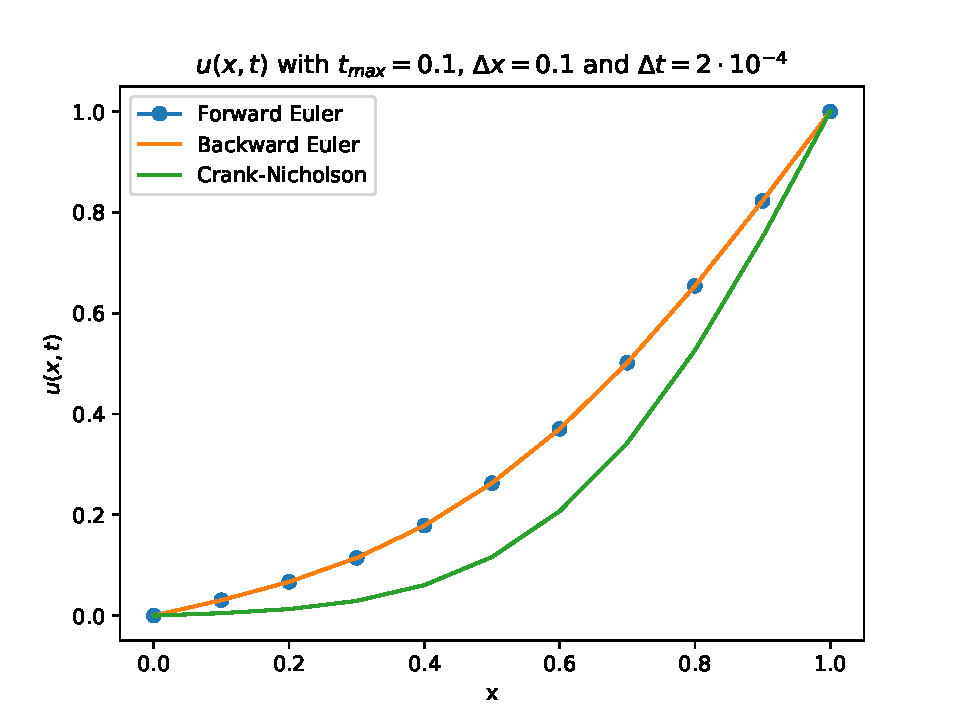
\includegraphics[width = 0.49\textwidth]{../plots/t2.pdf}}  
  	\subfigure[\ $t_2$]{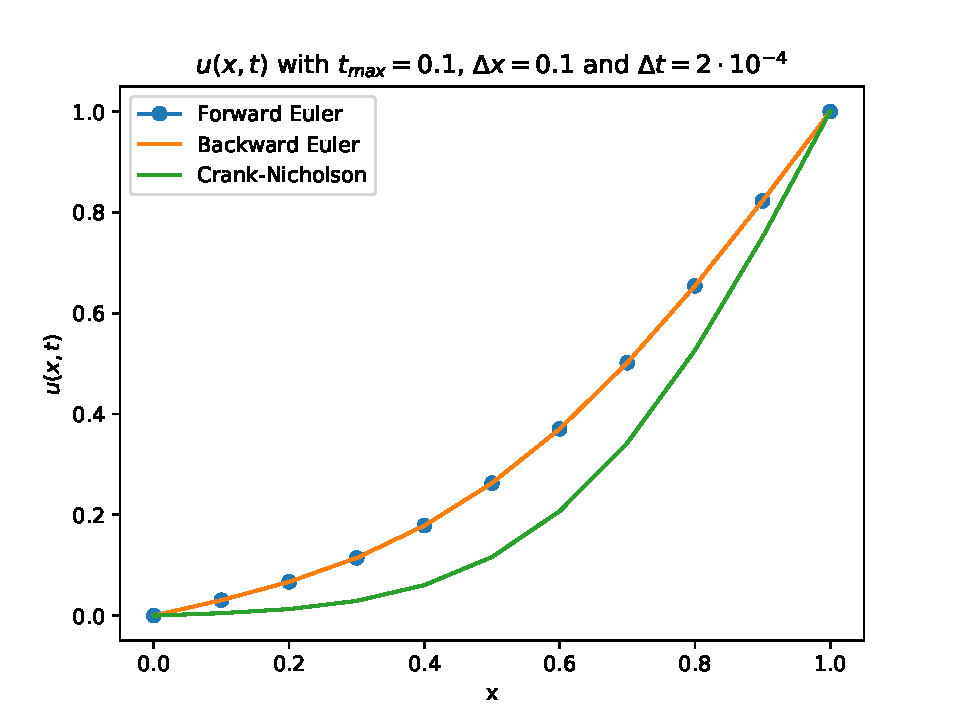
\includegraphics[width = 0.49\textwidth]{../plots/t1.pdf}}
  	\caption{\label{fig:5c}Comparison of $t_1$ and $t_2$.}
\end{figure}

\noindent Figure \ref{fig:5c} highlights the distribution of temperature at two different times. At $t_1$ the different schemes produce different distributions. Forward and backward euler line up closely, in contrast to the Crank-nicolson scheme. At $t_2$ the temperature distribution is linear and all the schemes line up closely. 

\begin{figure} [H]
	\centering
	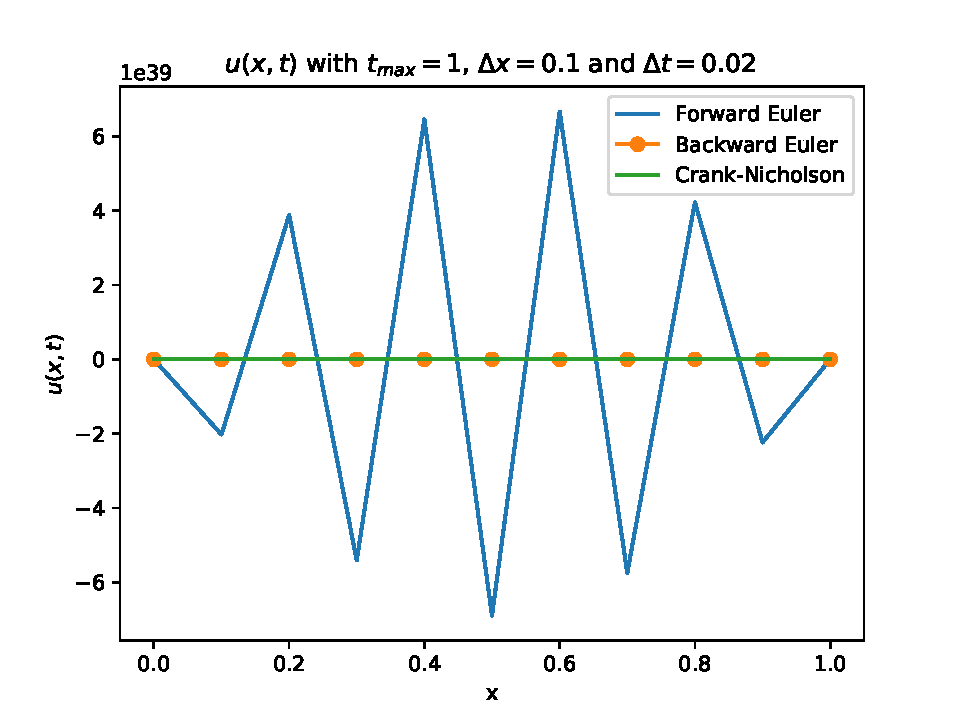
\includegraphics[width=0.48\textwidth]{../plots/unstable.pdf}
	\caption{\label{fig:unstable} Plot showing the effect of choosing unfavorable $\Delta x$ and $\Delta t$}
\end{figure}

\noindent As can be read out of Table \ref{truncstab}, the forward Euler scheme has a rigorous stability condition. Figure \ref{fig:unstable} shows a graphical representation of what happens when this condition is violated. 



\newpage
\section*{Discussion}

Table \ref{truncstab} shows that, even though the Euler forward method is easy to implement, there are serious limitations for the stability. The Euler backward and Crank-nicolson schemes are stable for all $\Delta x^2$ and $\Delta t^2$, but the implementation is more complicated. As the euler forward and Crank-nicolson uses a tridiagonal solver in the computation process, it is expected to be slower than the Euler forward scheme, which uses a more direct approach. Figure \ref{fig:unstable} shows that the forward Euler fluctuates a lot when the stability condition is violated. The stable schemes actually produce correct results, but are drowned by the fluctuations of the forward Euler. 
\\

\noindent In the one dimensional case, the system converges to an equilibrium. This is shown graphical in figure \ref{fig:5c}A and \ref{fig:5c}B. Given the boundary conditions $u(0,t)=0$ and $u(1,t)=1$ for all $t$, this can be translated to a one dimensional rod with  a heat source at $x=1$ and a heat sink at $x=0$. When starting the computation, the only point with a nonzero temperature is at $x=1$. The heat from this point then spreads through the rod. The heat rises quicker close to the heat source, as is shown in figure \ref{fig:5c}A, but will with time reach an equilibrium (figure \ref{fig:5c}B). It is important to note that the behavior of the system is entirely dependent on the boundary conditions. As an example, it would be possible to add another heat source at $x=0$ and the temperature would rise fast in the edges and slower in the middle. 
\\

\noindent The boundary conditions in the two dimensional case is depending on what kind of system being simulated. If the system in question is a two dimensional rod with a heat source at one end and heat loss at all the other edges, the temperature distribution would look like $enfigurejegikkehar$. If the system is the temperature distribution in the lithosphere, it is not expected to be much heat loss in the lateral direction. 








\newpage
\section*{Concluding remarks}





\newpage
\section*{References}


\end{document}
